The primary objective in machine learning (and therefore deep learning) is to perform well on new, unseen data.  The central challenge is finding the ideal balance between \textbf{overfitting} and \textbf{underfitting}.

\subsection{Rating Model Performance}

%start with \cite{Goodfellow-et-al-2016} (ch 5)

During the build process, a model is faced with a training set and measured against a test set.  With the training set, the model engages its optimization techniques (gradient decent) in order to minimiza a cost function (i.e. least squares).  The measurement of error that is reduced during optimization is known as the \textit{training error}.  When performance of new predictions is measured against the test set, the expected value of the error between predictions and actual text data is the \textit{test error} (commonly referred to as the \textit{generalization error}). \cite{Goodfellow-et-al-2016}

 When the model cannot obtain a sufficiently low test error, it is \textit{underfit}.  Often times, when a model is optimized toward a minimum training error, test error passes through a minimum rather than decreasing monotonically. \cite{mackay1992bayesian}  When the gap between the training error and test error is too great, the model is \textit{overfit}.  Somewhere between these extremes is the model's optimal \textit{capacity}.  Capacity is a model's ability to fit a wide variety of functions.  In linear regression, increasing the model's capacity would be to include polynomial terms or splines to shape the model beyond a straight line, as shown in Figure \ref{capacityviz}.  Neural networks have much higher complexity than ordinary least squares, making them extremely susceptible to overfitting.


%---begin R code for ggplot display of over- and underfit---
%--If this code is modified in R, push it to GotHub to Overeaf and re-copy and paste

\begin{comment}

\hypertarget{overfit-and-underfit}{%
\subsubsection{Overfit and Underfit}\label{overfit-and-underfit}}

\begin{Shaded}
\begin{Highlighting}[]
\CommentTok{\#Generate some noisy data}
\FunctionTok{set.seed}\NormalTok{(}\DecValTok{3}\NormalTok{)}
\NormalTok{a }\OtherTok{\textless{}{-}} \FunctionTok{runif}\NormalTok{(}\DecValTok{12}\NormalTok{, }\AttributeTok{min=}\DecValTok{0}\NormalTok{, }\AttributeTok{max=}\DecValTok{90}\NormalTok{)}
\NormalTok{c }\OtherTok{\textless{}{-}} \DecValTok{24}\SpecialCharTok{*}\FunctionTok{sin}\NormalTok{(.}\DecValTok{05}\SpecialCharTok{*}\NormalTok{a) }\SpecialCharTok{+} \FunctionTok{rnorm}\NormalTok{(}\FunctionTok{length}\NormalTok{(a),}\DecValTok{0}\NormalTok{,}\DecValTok{5}\NormalTok{) }\SpecialCharTok{+} \DecValTok{40}

\CommentTok{\#create data frame and base plot}
\NormalTok{df }\OtherTok{\textless{}{-}} \FunctionTok{data.frame}\NormalTok{(a,c)}
\NormalTok{model }\OtherTok{\textless{}{-}} \FunctionTok{ggplot}\NormalTok{(df, }\FunctionTok{aes}\NormalTok{(}\AttributeTok{x =}\NormalTok{ a, }\AttributeTok{y =}\NormalTok{ c)) }\SpecialCharTok{+}
        \FunctionTok{geom\_point}\NormalTok{(}\AttributeTok{size =} \DecValTok{3}\NormalTok{, }\AttributeTok{color =} \StringTok{"purple"}\NormalTok{) }\SpecialCharTok{+}
        \FunctionTok{ylim}\NormalTok{(}\DecValTok{30}\NormalTok{,}\DecValTok{80}\NormalTok{) }\SpecialCharTok{+}
        \FunctionTok{theme\_minimal}\NormalTok{()}


\CommentTok{\# underfit model}

\NormalTok{model }\SpecialCharTok{+}
    \FunctionTok{stat\_smooth}\NormalTok{(}\AttributeTok{method =}\NormalTok{ lm,}
              \AttributeTok{formula =}\NormalTok{ y }\SpecialCharTok{\textasciitilde{}} \FunctionTok{poly}\NormalTok{(x,}\DecValTok{1}\NormalTok{),}
              \AttributeTok{fullrange =}\NormalTok{ T,}
              \AttributeTok{color =} \StringTok{"turquoise"}\NormalTok{,}
              \AttributeTok{se =}\NormalTok{ F)}

\CommentTok{\# overfit model}

\NormalTok{pol }\OtherTok{\textless{}{-}} \DecValTok{9} \CommentTok{\# polynomial order}
\NormalTok{model }\SpecialCharTok{+} 
    \FunctionTok{stat\_smooth}\NormalTok{(}\AttributeTok{method =}\NormalTok{ lm,}
              \AttributeTok{formula =}\NormalTok{ y }\SpecialCharTok{\textasciitilde{}} \FunctionTok{poly}\NormalTok{(x,pol),}
              \AttributeTok{fullrange =}\NormalTok{ T,}
              \AttributeTok{color =} \StringTok{"turquoise"}\NormalTok{,}
              \AttributeTok{se =}\NormalTok{ F)}
\end{Highlighting}
\end{Shaded}

\end{comment}

%-----end R code snippet--------------------

\begin{figure}[H]
    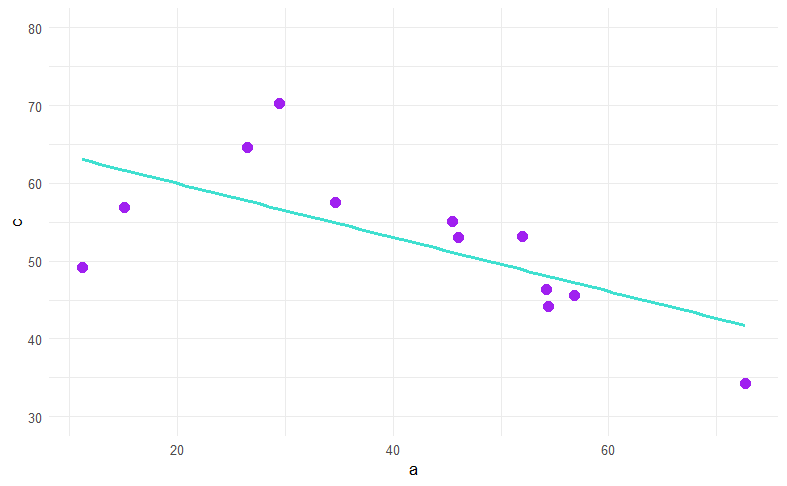
\includegraphics[width=0.5\linewidth]{Figures/underfit.png}
    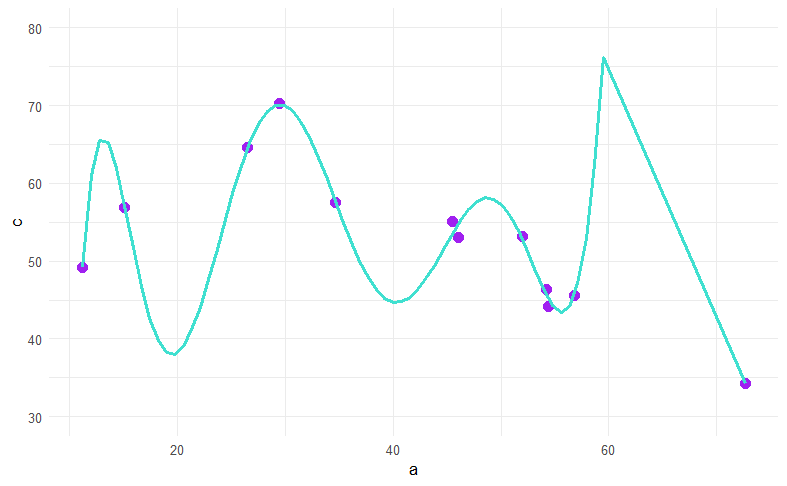
\includegraphics[width=0.5\linewidth]{Figures/overfit.png}
    \vspace{-20pt}
    \caption{\footnotesize{The regression model to the left has minimal capacity.  It underfits the data. The model to the right depicts an overfitting model.}}
    \label{capacityviz}
\end{figure}


- \textbf{Generalization}


\subsection{Addressing Model Performance}

There is no one way to set the dials of a neural network.  Generally, they are established by trial and error, train/test split, or more sophisticated techniques as cross-validation to compare networks trained with different parameter values. \cite{mackay1992practical}  The technique to improve model performance



\textbf{Regularization} is really any modification made to the learning process that aims to reduce test error (but not training error) \cite{Goodfellow-et-al-2016}


\textit{Early stopping} is when the optimization algorithm is halted before the test error increases too much.  It is hoped that the algorithm stops at an optimal model capacity.

\textit{Dropout} is \cite{srivastava2014dropout}

\textit{Weight decay} is the neural network equivalent to ridge regression in machine learning.  For more information on regularization techniques in traditional machine learning, consult \cite{Goodfellow-et-al-2016}  Weight decay is when a  term is added to the optimizer to penalize (often larger) weights in hopes to achieve a smoother fit. \cite{mackay1992practical}  For example, suppose a network architecture $A$ is defined for a model.  This architecture contains the specifications of the number of layers, neurons in each layer, activation functions, and available connections between layers.  The function mapping is defined as $\hat{y}(x^m;w,A)$.  If the gradient descent algorithm is used to reduce the following error function of the data $E_D$:
$$
E_D(D|w,A) = \sum_m \frac{1}{2} [\hat{y}(x^m;w,A) - y^m]^2
$$

the learning algorithm sets to reduce $E_D$ with the impementation of a \textit{regularizer} term for the weights $E_W$.  This regularizer can be defined as the following:
$$
E_W(w|A) = \sum_i \frac{1}{2} w_i^2
$$

The full optimization algorithm that uses weight decay then becomes:
$$
F = \alpha E_W(w|A) + \beta E_D(D|w,A)
$$
Where $\alpha$ and $\beta$ are "black box" parameters. \cite{mackay1992practical}  $\alpha$ is a control parameter known as the \textit{regularizing constant} (commonly referred to as the decay rate) and $\beta$ is the learning rate (step size).  Rules of thumb exist for setting these control parameters, and cross-validation can be applied to determine their optimal values as well.  In a later section, Bayesian methods will be applied to offer another method to determining $\alpha$ and $\beta$.


\subsection{Example: Tohoku Earthquakes}

%---Pathway to earthwuakes_lm_example R code
\subfile{earthquakes_lm_example}



\subsection{Quantification of Uncertainty}

Determining uncertainty in neural networks is not as simple as applying error bounds on the estimation.  Further construction is necessary to determine the level of confidence in a deep network's abilities, which stem from several methods.  The methods discussed here come from (H. M. Dipu Kabir, et.al) \cite{8371683}.  Thorough notation and detail will be spared as this thesis is not a comprehensive examination of uncertainty tactics.  Rather, methods will be discussed in their elementary form to illustrate the ease of using Bayes as an alternative.

The \textit{Delta method} is one which uses the Taylor expansion of the regression function to approximate the covariance matrix of the outputs.  More information can be found in \cite{nilsen2022epistemic} and \cite{hwang1997prediction}.  It is found that the covariance matrix grows quadratically with the number of parameters, making it extremely computationally costly to calculate, store, and use.  Delta also assumes normality and homogeneity, which limits its use in practice.  Further, when early stopping is used to train a network to prevent overfitting, the delta method results in very wide prediction intervals.

The \textit{Mean Variance Estimation Method (MVEM)} uses a dedicated neural network to obtain the mean in tandem with the network geared toward finding the variance.  The network to find the mean ($NN_{\hat{y}}$) is trained, followed by the network to estimate the variance ($NN_{\sigma}$) based on the parameter values of the first network.  This method allows extreme flexibility to account for heteroscedastic variance of target predictions.  There are no restrictions on the architectures of the two networks; they do not even have to be the same.  Error bounds can be calculated based on the estimated variance of the secondary neural net.  The main drawback to MVEM is that it assumes ($NN_{\hat{y}}$) accurately estimates the target values $y_i$ because ($NN_{\sigma}$) uses it to calculate its parameter values.  This can make for over- or underestimated error bounds.

The \textit{Bootstrap Method} is the most popular among traditional prediction interval uncertainty quantification.  The bootstrap algorithm comes in a variety of flavors (smooth,
parametric, wild, pairs, residual, Gaussian process, block
bootstraps ets.); neural network bootstrapping often uses pairs, although residual bootstrapping is often applied to neural net residuals.  This is usually done in either of two ways:  The first is to generate bootstrapped pairs by sampling with replacement the original training data and generate estimates from the trained neural network on each iteration of bootstrap pairs.  The second is to generate $B$ training data sets with bootstrap resampling and build $B$ neural network models from it.  The mean and variance of all point estimates from each neural network is calculated and used to create the model uncertainty.  The second method is obviously computationally costly, but the first can be too depending on the size of the data.  Neural networks often need a lot of data to produce adequate results.

Each of these methods has specialized variations to generate the most useful measurements of uncertainty; even to begin with it is only a start.  Each has been shown to have its own preference over others and pitfalls.  Indeed, as if building a neural network was not complex enough, the additional computations to deliver insight to the confidence of a network's predictions can be quite cumbersome. At the apotheoses of this thesis, it will be shown that applying Bayesian techniques to building a deep learning model yields uncertainty measures built right into the model itself.  The next section will review some introductions to Bayesian Statistics.